\section{量子カオス \label{app:quantum_chaos}}

\subsection{はじめに: カオスとは何か}
カオスの分野は19世紀末のヘンリ・ポアンカレによる3体問題に関する研究に始まる\cite{masoliver}。
2つの質点が互いに内力のみで相互作用し、外力が存在しないような2質点系は可積分系である。
そのような系の位相空間上の軌道は、一般に系の自由度の数だけ存在する保存量によって決まる多様体から
はみ出る事がなく、安定である。
一方、ポアンカレによって3質点系では摂動展開した級数の収束性は証明不可能である事が示された。
この問題を我々の太陽系に当てはめると、「太陽系は本当に安定な系か?」という興味深い
(そして少し不安になるような(?))問いとなる。
しかし我々の太陽系は観測上ケプラーの法則に非常に精度良く従っている。
ケプラーの法則は根本的に2質点系の可積分性から演繹されるものであるため、
太陽系のような多体系がこの法則に従うのは今日でも解消されていない謎の1つとなっている。

我々の住む世界には多くの場面においてカオスが顔を表す。
上述したような3つ以上の惑星を含む系の運動に始まり、化学反応、病気の広がり方、
インターネットや経済学にも現れる\cite{masoliver}。
一方、可積分系は非可積分系に比べて知られているものが非常に少ない。
可積分系という単語は、ハミルトン形式の力学において次のようにして定義される:
系の自由度を$n$とする。
この時、運動の定数$I_i(\vec{q}, \vec{p}) = \mathrm{const}$が$n$個あり、かつ
\begin{align}
	[I_i, I_j]_{\mathrm{poisson}} = 0
\end{align}
を満たす時、系は可積分性を持つという。
ここで$[,]_{\mathrm{poisson}}$は
\begin{align}
	[f,g]_{\mathrm{poisson}} = \sum_{i = 1}^{n}\left(
		\frac{\partial f}{\partial q_i}\frac{\partial g}{\partial p_i}
		- \frac{\partial f}{\partial p_i}\frac{\partial g}{\partial q_i}
	\right)
\end{align}
で与えられるポアソン括弧である。
ポアンカレによって、ほとんどの力学系は運動の定数としてエネルギーしか持たない事が示された\cite{masoliver}。
つまり、これらの系は自由度が$n=1$でなければ可積分系とはならない。
従って、$n \geq 2$となるようなほとんどの系は可積分系ではないと言える。

例として3次元空間内における$N$体問題を考えると、系の自由度が$3N$であるのに対して、
ポアソン括弧の意味で互いに可換となるような運動の定数は6つしかない。
故に$N=2$の時のみ可積分系となるのであり、それより多い数の物体が存在すると最早可積分系ではなくなる。

カオス系の最も簡易な定義は次のように与えられる:
ある1つの運動を、初期条件をわずかに変えて時間発展させた時、
運動の軌跡が初期条件によって大きく異なるような系をカオス系という。
この定義はいわゆるバタフライ効果である。
しかし古典カオスにおいて、これは寧ろ証明されるものであり、
より根本的かつ数学的に厳密な定義が複数存在する\cite{hsiao}:
1つは位相的推移性(topological transitivity)を持つ写像が存在する事である。
つまり、運動を表す状態空間(例えば位相空間)
$\mathcal{M}$上で作用する写像$f: \mathcal{M}\to\mathcal{M}$があり、
任意の2つの開集合$U, V$に対して$f^N(U)\cap V \neq \emptyset$となるような
自然数$N\in\mathbb{N}$が存在するというものである。
ここで$f^N(U) = f(f(\cdots f(U) \cdots ))$である。
もう少し直感的な言葉を使うなら、ある時点での任意の状態に対して、それに限りなく近づくような軌道が
状態空間$\mathcal{M}$内に必ず存在するという事でもある。
2つ目は状態空間$\mathcal{M}$内に周期的な点からなる稠密部分集合が存在する事である
\footnote{位相(\textit{topological})空間$X$の部分集合$A$が$X$において稠密であるとは、
	$x\in X$の任意の近傍$U(x)$が$U(x)\cap A \neq \emptyset$を満たす事を言う。
	等価な定義として、$A$を含む$X$の閉集合が$X$自身しかない時、$A$は稠密であるというものもある。}。
つまり、全ての状態$x\in\mathcal{M}$それぞれに限りなく近い点$y$が存在し、
$y$はある周期的な軌道に乗ったものである。
これらの定義は互いに等価な内容である。

古典カオスが位相空間を用いた厳密な定義を持つ一方で、量子カオスにはそのような定義が存在しない。
これは、量子系は不確定性原理により正準共役な変数が可換でなくなるため、
位相空間上の軌道という概念は最早意味を成さない事に起因する。

量子カオスの伝統的な研究手法では対応原理を使用する: カオス系として知られている
古典系を用意し、それを単純に量子化するのである。
典型的な系は次のようなものである\cite{ullmo}: あるリング上に存在する粒子を考える。
その粒子はある一定時間ごとにデルタ関数的なポテンシャルにより強く加速される。
ハミルトニアンは
\begin{align}
	H(x, p) = \frac{p^2}{2} + V(x)\sum_{n=-\infty}^{\infty}\delta(t-n)
	\label{eq:kicked_rotor}
\end{align}
の様に与えられる。ここで$V(x) = -\frac{K}{4\pi^2}\cos(2\pi x)$はリング上の周期的ポテンシャルである。
この系は$V(x)$の大きさ$K$によって可積分系からカオス系へと転移するという特徴を持ち
(図\ref{fig:phase_space_of_kicked_rotor})、
系を量子化した後でも、この性質は伏見関数$\Psi(x, p)$を見る事により保たれている事を示せる。
\begin{figure}[ht]
	\centering
	\begin{tabular}{c}
		\begin{minipage}{0.33\hsize}
			\centering
			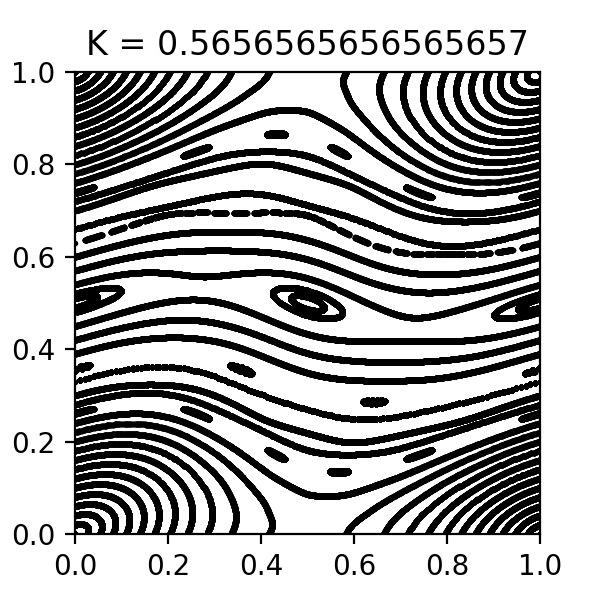
\includegraphics[width=5cm]{figures/figure7}
		\end{minipage}
		\begin{minipage}{0.33\hsize}
			\centering
			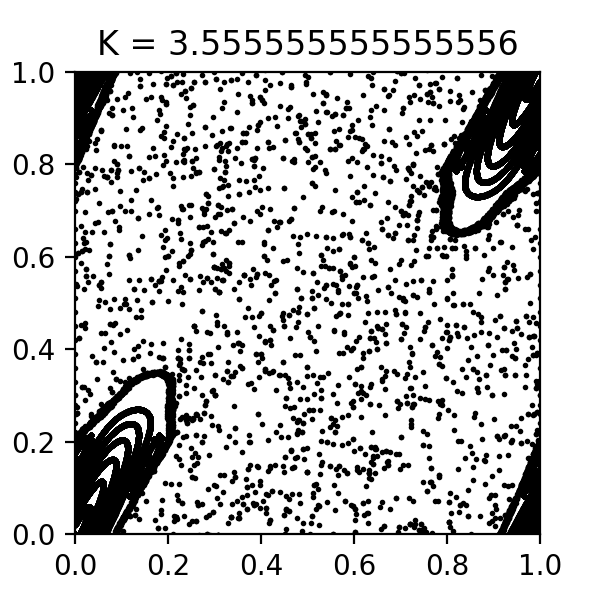
\includegraphics[width=5cm]{figures/figure44}
		\end{minipage}
		\begin{minipage}{0.33\hsize}
			\centering
			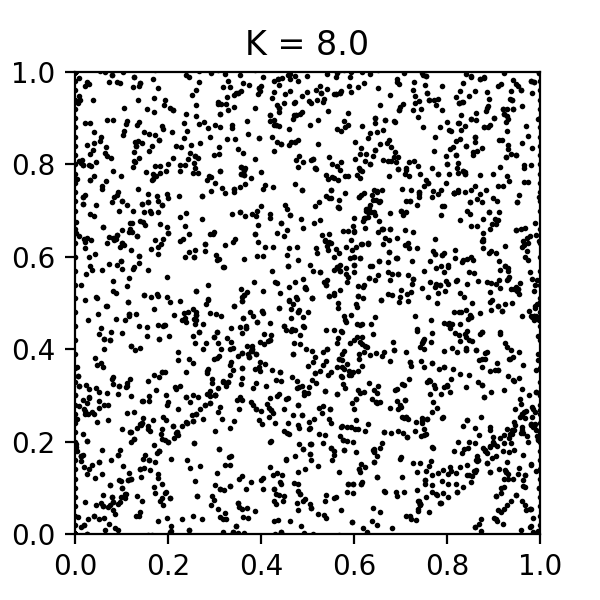
\includegraphics[width=5cm]{figures/figure99}
		\end{minipage}
	\end{tabular}
	\caption{\eqref{eq:kicked_rotor}式で与えられる系の位相空間上の軌道。
		横軸が$x$、縦軸が$p$である。$K$が大きくになるにつれて可積分性が消滅し
		カオスとなっていく。}
	\label{fig:phase_space_of_kicked_rotor}
\end{figure}

系の持つ量子カオス性を測定する道具として時間順序外相関関数
(out-of-time-order correlation function: OTOC)
というものがある:
\begin{align}
	C(t) \equiv -\average{[W(t), V(0)]^2}.
	\label{eq:OTOC}
\end{align}
ここで$W, V$はハイゼンベルグ描像での一般のエルミート演算子、そして
$\average{A} \equiv Z^{-1}\mathrm{tr}(e^{-\beta H}A)$である。
交換子$[W(t), V(0)]$は、時刻$t$における測定量$W$に対する$V(0)$による
摂動の効果を表し、その熱平均(thermal average)を取る事で影響の大きさを
測ったものが\eqref{eq:OTOC}式である。

量子カオスを調べる道具はもう1つ存在する。
量子カオスの性質にエネルギー固有値などのスペクトラムが統計的な振る舞いをするというものがある。
一方で可積分性を持つ量子系(対応する古典系が可積分系)のスペクトラムはランダムであり、
統計的な分布を持たない。
この事から量子カオスの性質を探る統計的手法としてスペクトラル統計が使われる。
用いる数学はランダム行列理論(Random Matrix Theory: RMT)である。
ランダム行列とは、その名の通りある確率分布に従う乱数を成分として持つ行列であり、
RMTはその統計的な性質を調べるものである。
重要な量として挙げられるものは複数あるが、特にSYK模型と関連が深いものは
スペクトラル形状因子(spectral form factor)$g(t)$である。
量子カオスを示す系ではスペクトラル形状因子は特有の構造を持ち、
その物理的起源を探求する事が主な研究課題となる。

以下ではOTOC及びスペクトラル統計について詳しく解説する。

\subsection{時間順序外相関関数}
OTOCは古典カオスのバタフライ効果の定義を量子論に拡張したものである。


\subsection{スペクトラル統計}

\pagebreak
